\documentclass{beamer}
\usepackage[utf8]{inputenc}

\usetheme{Madrid}
\usecolortheme{default}
\usepackage{amsmath,amssymb,amsfonts,amsthm}
\usepackage{txfonts}
\usepackage{tkz-euclide}
\usepackage{listings}
\usepackage{adjustbox}
\usepackage{array}
\usepackage{tabularx}
\usepackage{gvv}
\usepackage{lmodern}
\usepackage{circuitikz}
\usepackage{tikz}
\usepackage{graphicx}

\setbeamertemplate{page number in head/foot}[totalframenumber]

\usepackage{tcolorbox}
\tcbuselibrary{minted,breakable,xparse,skins}



\definecolor{bg}{gray}{0.95}
\DeclareTCBListing{mintedbox}{O{}m!O{}}{%
	breakable=true,
	listing engine=minted,
	listing only,
	minted language=#2,
	minted style=default,
	minted options={%
		linenos,
		gobble=0,
		breaklines=true,
		breakafter=,,
		fontsize=\small,
		numbersep=8pt,
		#1},
	boxsep=0pt,
	left skip=0pt,
	right skip=0pt,
	left=25pt,
	right=0pt,
	top=3pt,
	bottom=3pt,
	arc=5pt,
	leftrule=0pt,
	rightrule=0pt,
	bottomrule=2pt,
	toprule=2pt,
	colback=bg,
	colframe=orange!70,
	enhanced,
	overlay={%
		\begin{tcbclipinterior}
			\fill[orange!20!white] (frame.south west) rectangle ([xshift=20pt]frame.north west);
	\end{tcbclipinterior}},
	#3,
}
\lstset{
	language=C,
	basicstyle=\ttfamily\small,
	keywordstyle=\color{blue},
	stringstyle=\color{orange},
	commentstyle=\color{green!60!black},
	numbers=left,
	numberstyle=\tiny\color{gray},
	breaklines=true,
	showstringspaces=false,
}
%------------------------------------------------------------
%This block of code defines the information to appear in the
%Title page
\title %optional
{4.13.51}
%\subtitle{A short story}

\author % (optional)
{RAVULA SHASHANK REDDY - EE25BTECH11047}

 \begin{document}
	
	
	\frame{\titlepage}
	\begin{frame}{Question}
One of the diameters of the circle circumscribing the rectangle \(ABCD\) is given by
\begin{align*}
4y = x + 7.
\end{align*}

If \(\vec{A}=(-3,4)\) and \(\vec{B}=(5,4)\), find the area of the rectangle.

\end{frame}
\begin{frame}{Solution}
    \begin{align}
\vec{A}=\myvec{-3\\4},\quad \vec{B}=\myvec{5\\4}
\end{align}

Centre \(\vec{O}=\myvec{x\\y}\) satisfies
\begin{align}
\myvec{1 \\ 0}^T\vec{x}=1,\qquad \myvec{1 \\ -4}^T\vec{x}=-7
\end{align}

\begin{align}
\myvec{1 & 0\\ 1 & -4}\vec{x} &= \myvec{1\\-7}
\end{align}
\begin{align}
\myvec{1 & 0 & 1\\[4pt] 1 & -4 & -7}
\xrightarrow{R_2\rightarrow R_2-R_1}
\myvec{1 & 0 & 1\\[4pt] 0 & -4 & -8}
\xrightarrow{R_2\rightarrow (-\tfrac{1}{4})R_2}
\myvec{1 & 0 & 1\\[4pt] 0 & 1 & 2}
\end{align}
\end{frame}
\begin{frame}{Solution}
\begin{align}
    \vec{O}=\myvec{1\\2}
\end{align}

\begin{align}
\vec{C}&=2\vec{O}-\vec{A}=\myvec{2\\4}-\myvec{-3\\4}=\myvec{5\\0},\\
\vec{D}&=2\vec{O}-\vec{B}=\myvec{2\\4}-\myvec{5\\4}=\myvec{-3\\0}.
\end{align}
\begin{align}
\vec{B}-\vec{A}=\myvec{8\\0},\qquad
\vec{D}-\vec{A}=\myvec{0\\-4}.
\end{align}

\begin{align}
\text{Area} &= \big|\vec{B}-\vec{A}\times\vec{D}-\vec{A}\big|
= \left|\det\myvec{8 & 0\\[4pt]0 & -4}\right|
= |8(-4)-0| = 32.
\end{align}

\end{frame}
\begin{frame}[fragile]
\frametitle{C Code}
\begin{lstlisting}
    #include <stdio.h>
#include <math.h>

int main() {
    // Given points
    double A[2] = {-3, 4};
    double B[2] = {5, 4};

    // Solve equations for center
    // x = 1
    // x - 4y = -7
    double x = 1;
    double y = (x + 7) / 4.0;

    double O[2] = {x, y};
    printf("Center O = (%.2f, %.2f)\n", O[0], O[1]);
\end{lstlisting}
\end{frame}
\begin{frame}[fragile]
\frametitle{C Code}
\begin{lstlisting}
    // Opposite vertices
    double C[2] = {2*O[0] - A[0], 2*O[1] - A[1]};
    double D[2] = {2*O[0] - B[0], 2*O[1] - B[1]};

    printf("C = (%.2f, %.2f)\n", C[0], C[1]);
    printf("D = (%.2f, %.2f)\n", D[0], D[1]);

    // Side vectors
    double AB[2] = {B[0]-A[0], B[1]-A[1]};
    double AD[2] = {D[0]-A[0], D[1]-A[1]};

    // Cross product (2D determinant)
    double area = fabs(AB[0]*AD[1] - AB[1]*AD[0]);
    printf("Area of rectangle = %.2f\n", area);

    return 0;
}
\end{lstlisting}
\end{frame}
\begin{frame}[fragile]
\frametitle{Python Direct}
\begin{lstlisting}


import numpy as np
import matplotlib.pyplot as plt
from numpy import linalg as LA


# local imports
from libs.line.funcs import *
from libs.triangle.funcs import *
from libs.conics.funcs import circ_gen

# Given points
A = np.array([-3,4]).reshape(-1,1)
B = np.array([5,4]).reshape(-1,1)

# Centre O lies on x=1 and x-4y=-7
x = 1
y = (x+7)/4
\end{lstlisting}
\end{frame}
\begin{frame}[fragile]
\frametitle{Python Direct}
\begin{lstlisting}
O = np.array([x,y]).reshape(-1,1)

# Opposite vertices
C = 2*O - A
D = 2*O - B

# Side vectors
AB = B - A
AD = D - A

# Area by cross product
area = abs(np.linalg.det(np.hstack((AB,AD))))
print("Area of rectangle =", area)

# Circumcircle radius
r = LA.norm(A - O)
\end{lstlisting}
\end{frame}
\begin{frame}[fragile]
\frametitle{Python Direct}
\begin{lstlisting}
# Circle points
x_circ = circ_gen(O.flatten(), r)

# Plotting
rect_coords = np.hstack((A,B,C,D,O))
labels = ['$A$','$B$','$C$','$D$','$O$']

plt.plot(x_circ[0,:], x_circ[1,:], label='Circumcircle')
plt.plot([A[0,0],B[0,0],C[0,0],D[0,0],A[0,0]],
         [A[1,0],B[1,0],C[1,0],D[1,0],A[1,0]],
         'k-',label='Rectangle')

plt.scatter(rect_coords[0,:], rect_coords[1,:])
\end{lstlisting}
\end{frame}
\begin{frame}[fragile]
\frametitle{Python Direct}
\begin{lstlisting}
for i, txt in enumerate(labels):
    plt.annotate(f'{txt}({rect_coords[0,i]:.0f},{rect_coords[1,i]:.0f})',
                 (rect_coords[0,i], rect_coords[1,i]),
                 textcoords="offset points", xytext=(-10,5), ha='center')

ax = plt.gca()
ax.spines['top'].set_color('none')
ax.spines['right'].set_color('none')
ax.spines['left'].set_position('zero')
ax.spines['bottom'].set_position('zero')

plt.grid()
plt.axis('equal')
plt.legend()
plt.show()
\end{lstlisting}
\end{frame}
\begin{frame}[fragile]
\frametitle{Python Shared}
\begin{lstlisting}

import numpy as np
import matplotlib.pyplot as plt
from numpy import linalg as LA
import ctypes

# local imports
from line.funcs import *
from triangle.funcs import *
from conics.funcs import circ_gen

# Load C library
lib = ctypes.CDLL('./rect.so')
lib.rect_area.restype = ctypes.c_double
c_area = lib.rect_area()

# Given points
A = np.array([-3,4]).reshape(-1,1)
B = np.array([5,4]).reshape(-1,1)
\end{lstlisting}
\end{frame}
\begin{frame}[fragile]
\frametitle{Python Shared}
\begin{lstlisting}
# Centre O
x = 1
y = (x+7)/4
O = np.array([x,y]).reshape(-1,1)

# Opposite vertices
C = 2*O - A
D = 2*O - B

# Side vectors
AB = B - A
AD = D - A

# Area via cross product in Python
p_area = abs(np.linalg.det(np.hstack((AB,AD))))

print("Area from C (ctypes)   =", c_area)
print("Area from Python      =", p_area)
\end{lstlisting}
\end{frame}
\begin{frame}[fragile]
\frametitle{Python Shared}
\begin{lstlisting}
# Circumcircle radius
r = LA.norm(A - O)
x_circ = circ_gen(O.flatten(), r)

# Plot
rect_coords = np.hstack((A,B,C,D,O))
labels = ['$A$','$B$','$C$','$D$','$O$']

plt.plot(x_circ[0,:], x_circ[1,:], label='Circumcircle')
plt.plot([A[0,0],B[0,0],C[0,0],D[0,0],A[0,0]],
         [A[1,0],B[1,0],C[1,0],D[1,0],A[1,0]],
         'k-',label='Rectangle')

plt.scatter(rect_coords[0,:], rect_coords[1,:])
\end{lstlisting}
\end{frame}
\begin{frame}[fragile]
\frametitle{Python Shared}
\begin{lstlisting}
for i, txt in enumerate(labels):
    plt.annotate(f'{txt}({rect_coords[0,i]:.0f},{rect_coords[1,i]:.0f})',
                 (rect_coords[0,i], rect_coords[1,i]),
                 textcoords="offset points", xytext=(-10,5), ha='center')

ax = plt.gca()
ax.spines['top'].set_color('none')
ax.spines['right'].set_color('none')
ax.spines['left'].set_position('zero')
ax.spines['bottom'].set_position('zero')

plt.grid()
plt.axis('equal')
plt.legend()
plt.show()

\end{lstlisting}
\end{frame}
\begin{frame}{Plot}
\begin{figure}
    \centering
    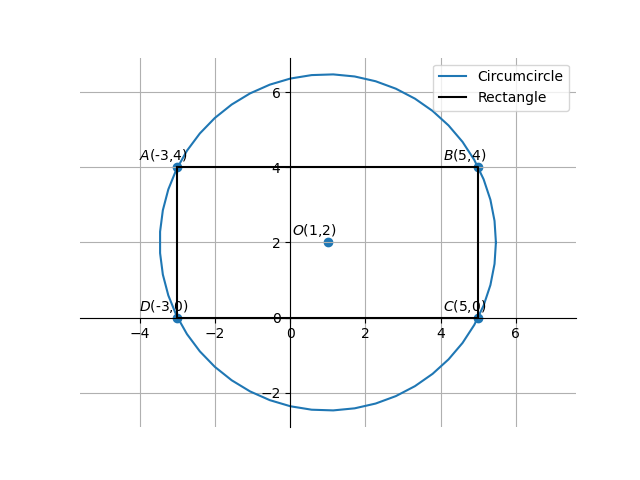
\includegraphics[width=0.75\linewidth]{figs/fig1.png}
    \caption{}
    \label{fig:placeholder}
\end{figure}
    
\end{frame}
\end{document}
